\section{Marco teórico}
El potencial de Lennard-Jones describe la energía potencial de interacción entre dos átomos o moleculas netros sujetos a dos fuerzas distintas, una fuerza que tiene mayor acción cuando la distancia entre las dos sistemas es grande y la otra fuerza de interacción tiene una mayor acción a corta distancia. Este potencial tiene la siguiente forma:
\begin{equation}
    \label{Potencial de Lennard-Jones}
    V(r) = 4 \epsilon \left[\left(\frac{\sigma}{r} \right)^{12} - \left(\frac{\sigma}{r} \right)^6 \right]
\end{equation}
donde:
\begin{itemize}
    \item $V$ es el potencial intermolecular entre dos átomos o partículas.
    \item $\epsilon$ es la profundidad del valle que define que tan fuerte es la atracción entre partículas.
    \item $\sigma$ es la distancia a la cual el potencial entre dos partículas es igual a cero.
    \item $r$ es la distancia de separación entre dos partículas
\end{itemize}
Los parámetros $\epsilon$ y $\sigma$ son ajustados para reproducir datos experimentales o pueden ser dedudidos de resultados a partir de cálculos de química cuántica. La fígura \ref{Potencial de Lennard-Jones} es el potencial de Lennard-Jones con $\epsilon=1$ y $\sigma=1$.\\
En donde expone una gráfica de potenciales universales para estructuras de gráfito, y la que tenemos se asemeja en comportamiento a pesar de no tener la estrucura de un grafito.
Teniendo el potencial de la ecuación \ref{Potencial de Lennard-Jones}, podemos deducir la fuerza, ya que esta puede ser deducida a partir de aplicar el gradiente a la función $V(r)$, teniendo así la siguiente expresión:
\begin{equation}
    \label{eq:fuerzateo}
    \vec{F}(r)= 48\epsilon \left(\frac{\sigma^{12}}{r^{13}}- \frac{1}{2}\frac{\sigma^6}{r^7} \right) \hat{r}
\end{equation}
reescribiendo las ecuaciones \ref{Potencial de Lennard-Jones} y \ref{eq:fuerzateo} para tener la suma de estas en un sistema de n particulas se tiene lo siguiente:
\begin{equation}
    \label{eq:pot-n}
    U_t=\left\langle\sum_{i=1}^N \sum_{j<i}^N V_i,j(|r_j-r_i|)\right\rangle_t
\end{equation}
\begin{equation}
    \changefontsizes{9pt}
    \label{eq:f-n}
    F_i = \frac{48}{\sigma^2} \sum_{j \ne i} \left[\left(\frac{\sigma}{r_{ij}}\right)^{14}-\frac{1}{2}\left(\frac{\sigma}{r_{ij}} \right)^8  \right] (r_j-r_i)
\end{equation}
\begin{figure}[H]
    \centering
    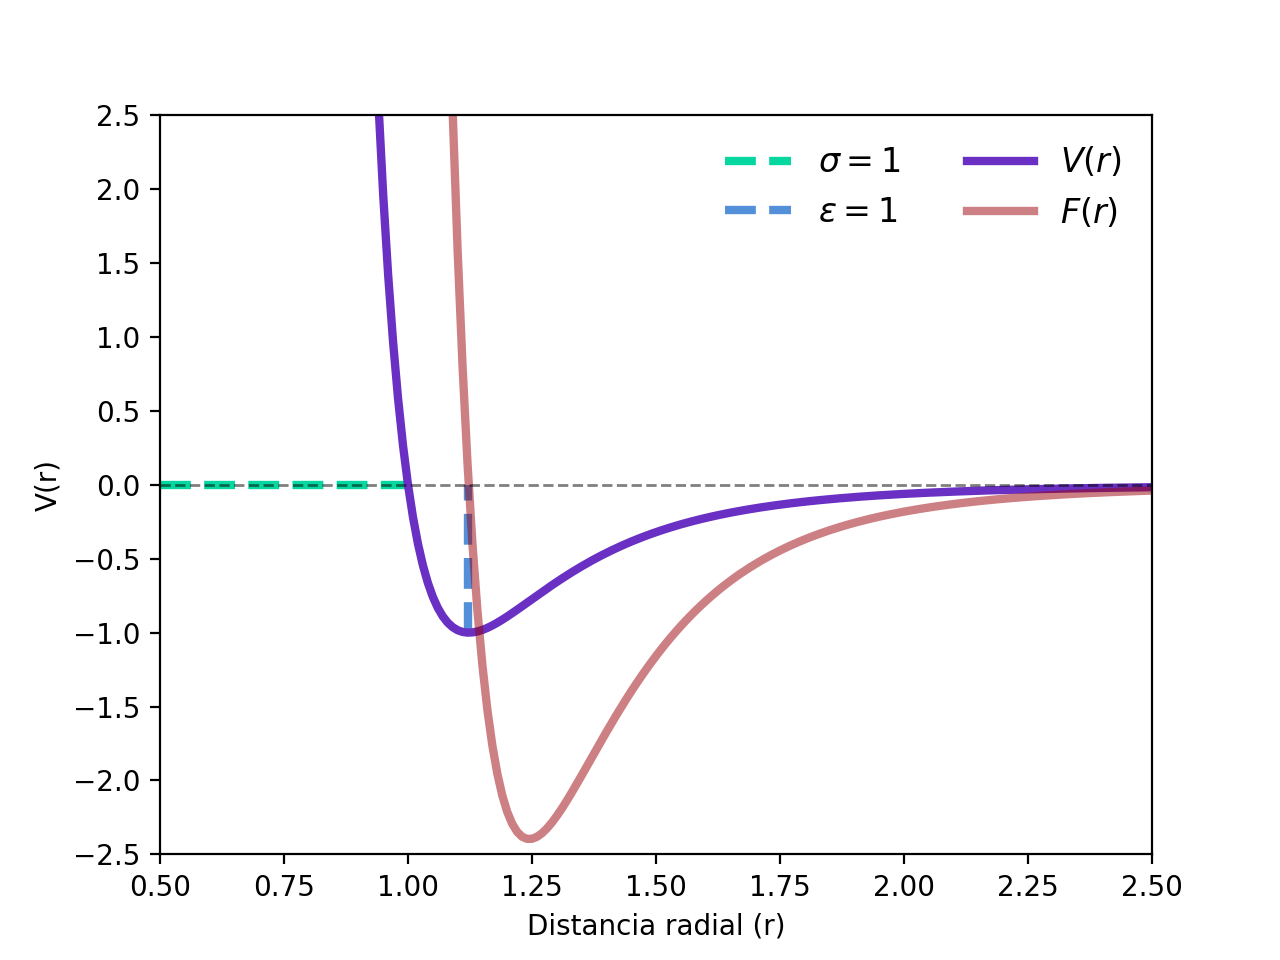
\includegraphics[scale=0.42]{../Graphics/Potencial.png}
    \caption{Potencial y fuerza de Lennard-Jones}
    \label{fig:pot-len-jones}
\end{figure}
\begin{table*}
    \centering
    \begin{tabular}{cp{1cm}p{0.5cm}ccccc}
        \hline
        Número de átomos & $\epsilon_{LJ}$ & $\sigma_{LJ} $ & $\rho $ & Número de pasos & T\textsubscript{0} & $\mu$ &$\sigma^2$\\ \hline
        \multirow{2}{*}{784} &\multirow{2}{*}{1} &\multirow{2}{*}{1}  &\multirow{2}{*}{Variable$^{*}$}  &\multirow{2}{*}{$2x10^{3}$} & \multirow{2}{*}{0.6} & \multirow{2}{*}{0}  & \multirow{2}{*}{1}\\
          & & & & & \\ \hline
    \end{tabular}
    \caption{Parámetros para las diferentes simulaciones, los valores tomados para las densidades fueron: 0.4, 0.5, 0.6, 0.7}
    \label{table:parametros}
\end{table*}
Teniendo ya la dinámica se este sistema podemos ir monitoreando la energía cinética de la siguiente manera:
\begin{equation}
    \label{eq:kin-n}
    T_t=\left\langle \sum_{i=1}^N \frac{1}{2}m|v_i(t)|^2\right\rangle
\end{equation}
por lo tanto, la energía total para un tiempo t será:
\begin{equation}
    \label{eq:e-tot}
    E_t=T_t+U_t
\end{equation}
El termostato de Andersen introduce un elemento estocastico a la temperatura teniendo colisiones aleatorias en las moleculas dentro de un 
entorno imaginario con una temperatura dada. En la aproximación para una partícula, se toma su velocidad y es reasignada por un valor aleatorio
de la distribución Maxwell-Boltzmann para una temperatura dada:
\begin{equation}
    \wp(v_{qi})= \left(\frac{m_i}{2\pi k_\beta T} \right)^\frac{1}{2} exp\left(- \frac{m_i v_{qi}^2}{2k_\beta T} \right)
\end{equation}
La cual se asemeja a una distribución normal, la implementación de esta función dentro de la simulación se realizó con la siguiente ecuación:
\begin{equation}
    \changefontsizes{8pt}
    {v}'_i= \sigma^2 \sqrt{-2log(\chi_1)} \left(cos(2\pi \chi_2) + sin(2\pi \chi_2) \right) + \mu 
    \label{eq:gauss}
\end{equation}
donde la variable $\chi_i$ es un número aleatorio de una distribución uniforme. Comprobando que esta función nos regresa una distribución normal
se probo con 100,000 valores y se obtuvó el siguiente histograma:
\begin{figure}[H]
    \centering
    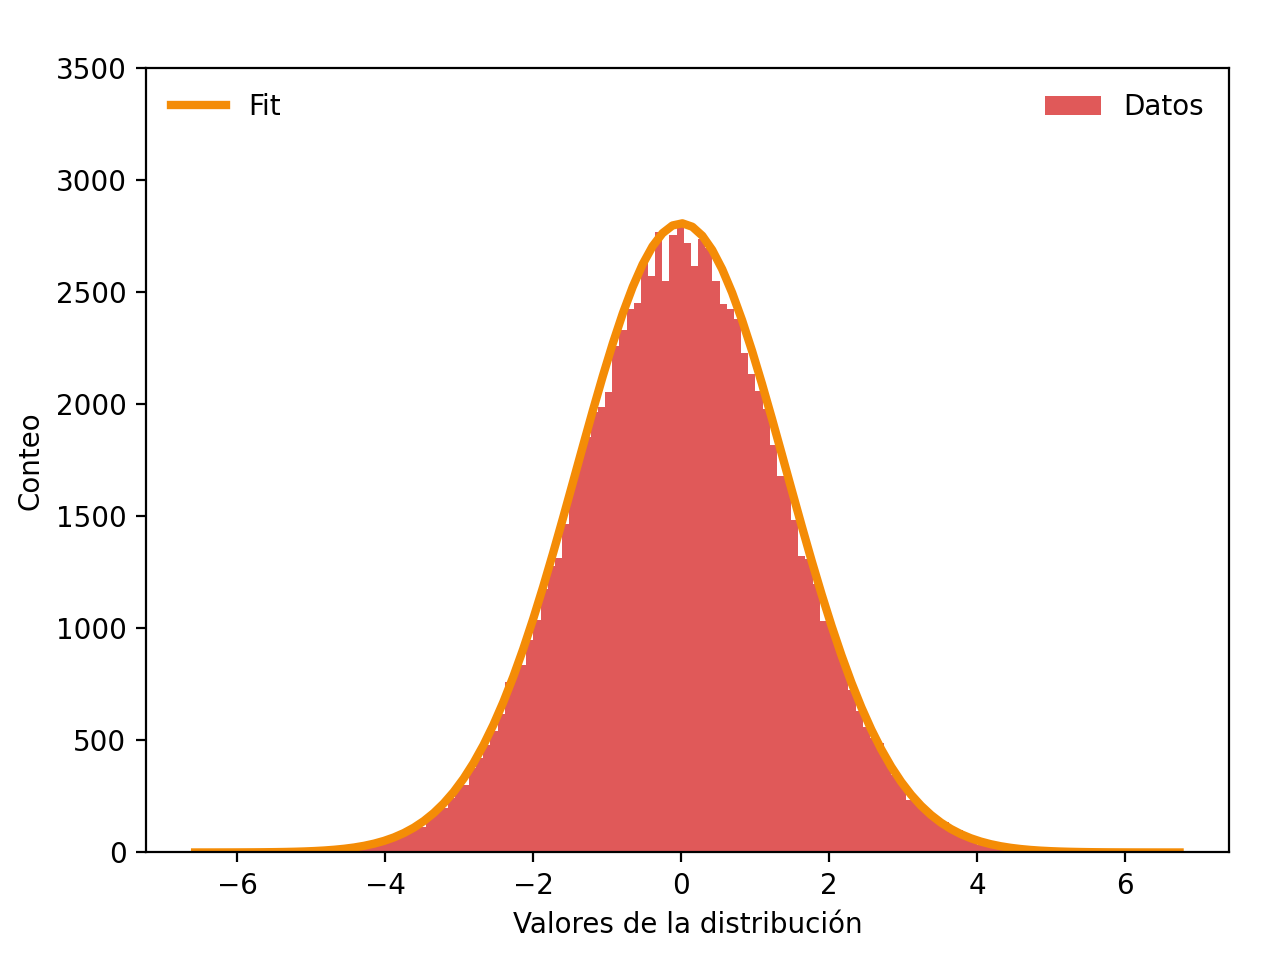
\includegraphics[scale=0.4]{../Graphics/norm.png}
    \caption{Distribución de valores que arroja la función \ref{eq:gauss} junto con su fit a una distribución normal.}
    \label{fig:gauss}
\end{figure}